\section{Introduction}
\subsection{The canonical example}
Let us consider the example from the abstract of water filtering through a porus medium, but this time in two dimensions. How do we model this? One might imagine that the medium consists of
many particles arranged (for simplicity) in an $n \times n$ square lattice and linked to each of their nearest neighbours. Clearly, this is the lattice on $\mathbb{Z}^2$.
To set up the problem, each of the particles will be expressed as a vertex in a graph and each of the links will be an edge. In the context of percolation, a vertex is called a site and an edge is
called a bond; these sites and bonds form a network.

\begin{definition}\label{def:bond}
  A vertex in a graph is referred to as a \textbf{bond}.
\end{definition}

\begin{definition}\label{def:site}
  A edge in a graph is referred to as a \textbf{site}.
\end{definition}

\begin{definition}\label{def:network}
  A graph is referred to as a \textbf{network}.
\end{definition}


So what does percolation actually mean? First we shall introduce the notion of open and closed sites and bonds and then we can discuss percolation.

\begin{definition}\label{def:open}
  A site or bond in a network is labeled \textbf{open} if it allows whatever we're considering to pass through.
\end{definition}

\begin{definition}\label{def:closed}
  A site or bond in a network is labeled \textbf{closed} if it doesn't allow whatever we're considering to pass through.
\end{definition}

And now for the percolation definitions.

\begin{definition}\label{def:sitepercolation}
  We say that we are considering \textbf{site percolation} if we let all of the sites in the network be open with probability $p \in [0, 1]$ and closed with probability $1-p \in [0, 1]$.
\end{definition}
\begin{definition}\label{def:bondpercolation}
  We say that we are considering \textbf{bond percolation} if we let all of the bonds in the network be open with probability $p \in [0, 1]$ and closed with probability $1-p \in [0, 1]$.
\end{definition}

Now that we've defined site and bond percolation, what's the problem that we're trying to solve? In the case of water being poured on a porus medium, we would like to know
whether there is an open path from the top of the network to the bottom.

\begin{definition}\label{def:open}
  We say that a path in a network is \textbf{open} if:
  \begin{itemize}
    \item when considering site perolation, every site in the path is open.
    \item when considering bond percolation, every bond in the path is open.
  \end{itemize}
\end{definition}

\begin{definition}\label{def:openly connected}
  Let $N=(V, E)$ be a network and let $A, B \in V$. The sites $A, B$ are \textbf{openly connected} if $\exists$ an open path connecting $A$ and $B$.
\end{definition}

\begin{definition}\label{def:openly disconnected}
  Let $N=(V, E)$ be a network and let $A, B \in V$. The sites $A, B$ are \textbf{openly disconnected} if $\nexists$ an open path connecting $A$ and $B$.
\end{definition}

The probability that an open path from the top of the network to the bottom exists depends on both our choices of both $p$ and $n$. As a result of our context, our value for $n$ should be
large---this is the case with most percolation models---but we shall use small $n$ for the sake of example and simplicity. Let us now fix $n$ and see what happens as we vary $p$. Obviously we have two trivial cases, $p=0$ and $p=1$,
where the network is completely openly disconnected and completely openly connected respectively.
What about when $p\in(0,1)$? Let's inspect three different values of $p$ on our network: $p=0.25$, $p=0.5$ and $p=0.75$ as shown in figures \ref{fig:p=0.25}, \ref{fig:p=0.5} and
\ref{fig:p=0.75} on page \pageref{fig:probabilities}.
As one might expect, as $p$ increases, so does the "connectedness" of the network; i.e. the probability of having an open path from the top of the network to the bottom increases
with $p$. Also, observe that as $p$ increases we also get larger "clusters" of open connected sites or bonds.

\begin{definition}\label{def:cluster}
  Let $N=(V, E)$ be a network. A \textbf{cluster} is a set of vertices, $C \subset V$, such that if $v_1, v_2 \in C$ then $v_1$ and $v_2$ are openly connected.
\end{definition}

\begin{definition}\label{def:cluster size}
  Let $N=(V, E)$ be a network and let $C \subset V$ be a cluster. The \textbf{size} of $C$, denoted by $|C|$, is the number of sites in the cluster.
\end{definition}

\begin{figure}[p]
  \centering
  \begin{subfigure}[b]{0.45\textwidth}
    \centering
    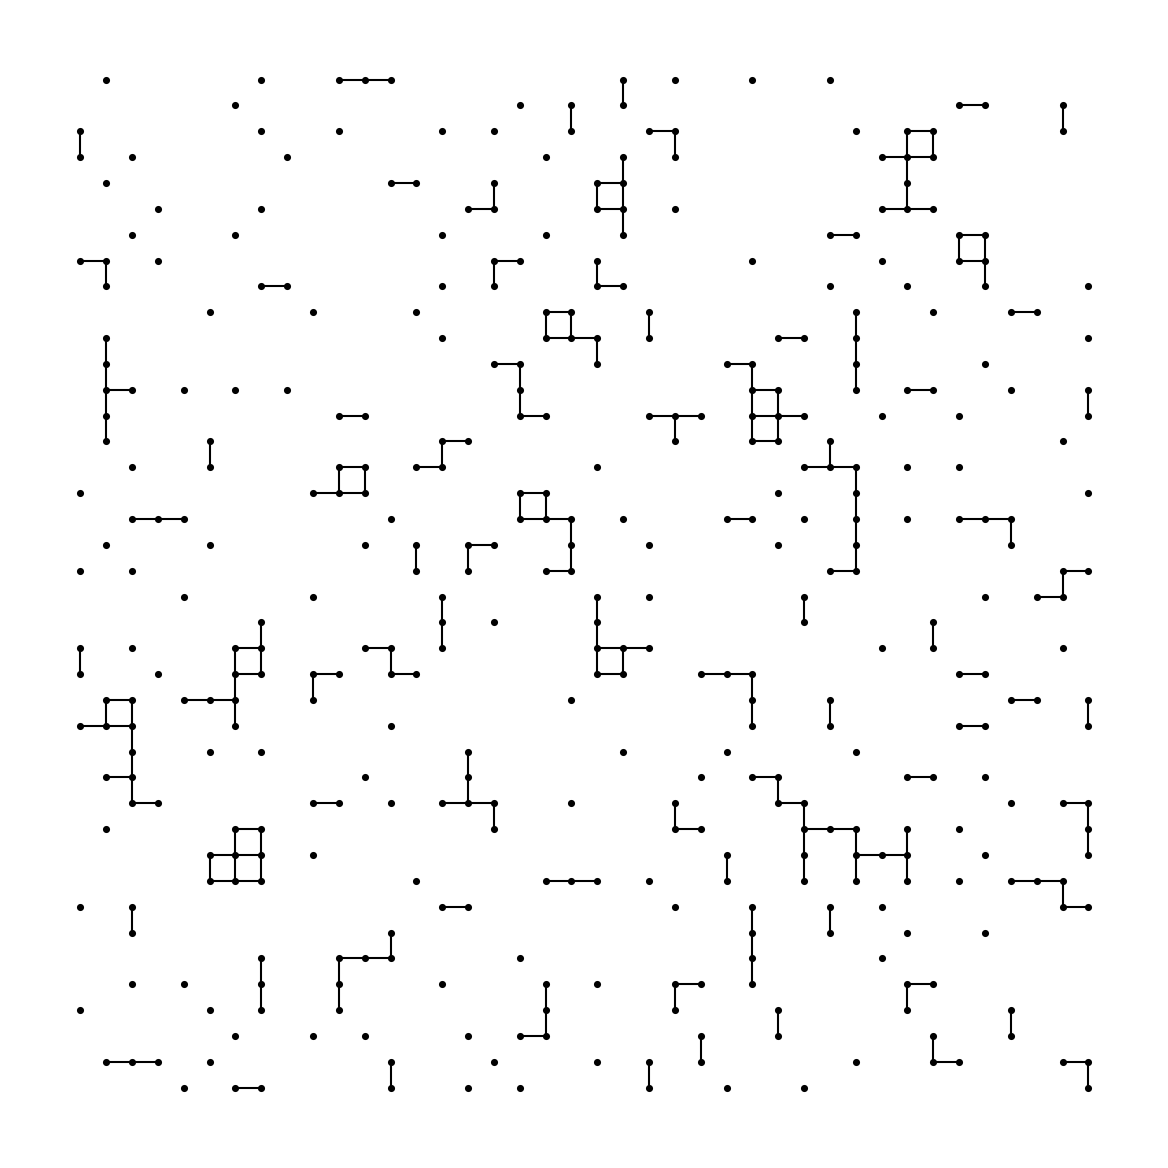
\includegraphics[width=\textwidth]{1/percolation1}
    \caption{$p=0.25$}
    \label{fig:p=0.25}
  \end{subfigure}
  \hfill
  \begin{subfigure}[b]{0.45\textwidth}
    \centering
    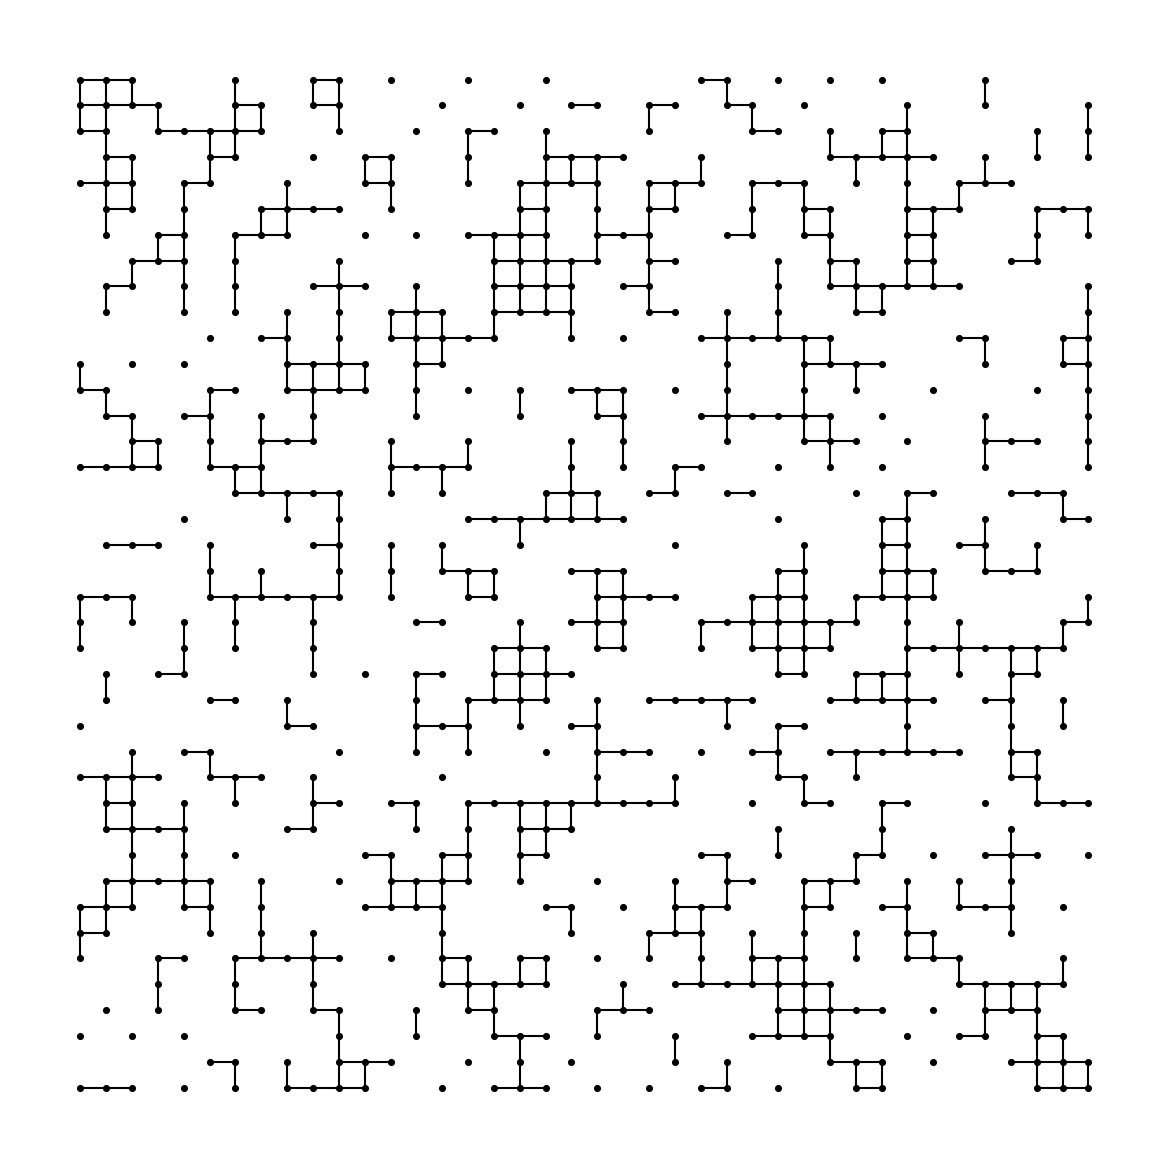
\includegraphics[width=\textwidth]{1/percolation2}
    \caption{$p=0.5$}
    \label{fig:p=0.5}
  \end{subfigure}
  \hfill
  \begin{subfigure}[b]{0.45\textwidth}
    \centering
    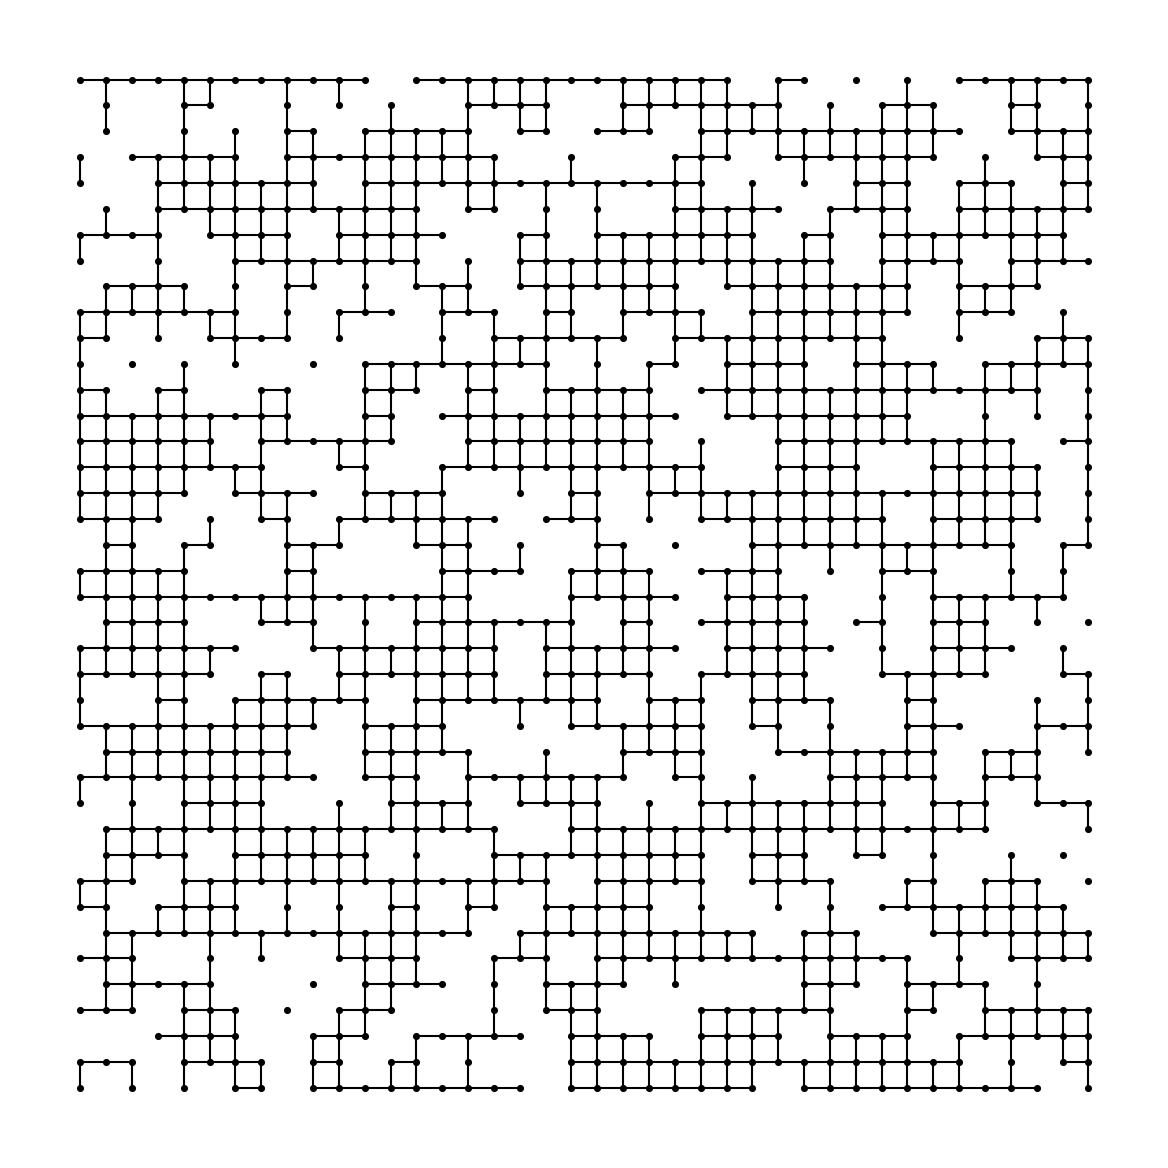
\includegraphics[width=\textwidth]{1/percolation3}
    \caption{$p=0.75$}
    \label{fig:p=0.75}
  \end{subfigure}
  \caption{Examples of percolation for $p\in(0,1)$.}
  \label{fig:probabilities}
\end{figure}

We will explore clusters in more detail in the next section, but for now let us introduce the idea of a critical probability. Although they don't exist in the finite cases, they do
exist in the infinite cases.

\begin{definition}\label{def:critical probability}
  Consider an infinite network, N. The critical probability, denoted $p_c$, is the probability such that an infinite cluster exists. The value of $p_c$ may not  be equal for site
  and bond percolation.
\end{definition}
